\subsection{Global validation of gene regulatory elements predicted by \egrine}
\label{section:tfbs:vs:regdb}

We compared the genome-wide locations of predicted GREs in the {\it
  E. coli} \egrine~model to experimentally mapped TF binding sites
from \rdb~(BindingSiteSet table, filtered for experimental evidence
and TFs with $\geq 3$ unique binding sites; a total of 88 TFs). We
considered a GRE to be a significant match to a TF if a significant
fraction ($q$-value $\leq 0.05$) of its predicted non-coding locations
overlapped with the known binding locations for a particular TF
(hypergeometric $p$-value $\leq 0.01$; see GRE definition in
Section~\ref{section:gres}). In cases where a GRE significantly
matched multiple TFs, only the most significant was reported.

We observed several instances where more than one GRE significantly
matched the same TF. We were unable to determine whether this was the
result of incomplete GRE clustering, ambiguities related to GRE
scanning, limitations of the experimental data itself, or a reflection
of subtle context-dependent variations in the binding preferences of
these TFs. Since we did not observe clustering of GREs that map to the
same TF upon re-clustering, we hypothesize that the observations may
have biological origins, \ie, reflect condition-dependent variations
in TF binding preferences that are the result, for example, of
co-activator/repressor interaction or small molecule binding. It is
interesting to note that TFs with the largest fraction of GRE matches
include transcriptional dual regulators, such as FlhDC and UlaR (\ie,
TFs with the ability to act as both activators and repressors). This
is consistent with the observation that these TFs have
context-dependent binding preferences. The complete set of
validations, for both TFs and $\sigma$-factors, is listed in Table~E4.

\subsection{Global validation of regulatory interactions predicted by \egrine}
\label{section:aupr:vs:regdb}

We assessed the ability of the \egrine\ model to correctly infer known
regulatory interactions using the \rdb\ database as a standard metric
for comparison. Comparison to the \rdb\ gold-standard is common
practice for evaluating model performance \cite{Marbach2012}. We
performed our evaluation with the version of \rdb~ used by the DREAM5
ensemble (based on \rdb\ release 6.8 \cite{Marbach2012}) so that we
could directly compare our results. The authors \cite{Marbach2012}
restricted the gold-standard to well-established interactions,
annotated in \rdb\ with the `strong evidence' classification. In all
cases, networks were integrated from predictions among the ensemble
using an approach similar to that of \cite{Marbach2012}, with subtle
variations noted in each section, below. To facilitate a direct
comparison, we reconstructed a new {\it E. coli} \egrine\ model using
the same DREAM5 expression consortium as was used for the original
DREAM5 competition (Section~\ref{section:dream5_data_compendium}). The
predictions of this model were used {\it solely} for global validation
and direct comparison with the DREAM5 community network, as described
in this subsection.

We performed two global evaluations of the {\it E. coli} \egrine: (1)
a comparison of the GREs detected in the model with experimentally
mapped TF binding sites in \rdb~(Section~\ref{section:tfbs:vs:regdb}),
and (2) a comparison of the predicted (TF $\rightarrow$ gene) regulation
in \egrine~with the gene regulatory network from
\cite{Marbach2012}. For (2), we computed predicted regulatory networks
from \egrine~in two ways: (a) direct (TF $\rightarrow$ target)
predictions from \nwinf~ (Section~\ref{sec:nwinf_network}, and (b) a
gene regulatory network derived from predicted GREs that were matched
to TFs in
\rdb~(Section~\ref{section:gre_grn_construction}). Construction of
each of these networks is described in detail below
(Section~\ref{sec:nwinf_network} and
Section~\ref{section:gre_grn_construction}). The methods for, and
results of the comparisons are described in
Section~\ref{sec:network_comparisons}.

\subsubsection{Conversion of \egrine~\nwinf~influence predictions into a GRN}
\label{sec:nwinf_network}

We computed a direct (TF $\rightarrow$ gene) inferred {\it E. coli}
gene regulatory network (GRN) from the \nwinf~predictions in the
\egrine~ensemble. As with the original EGRIN model \cite{Bonneau2007},
\nwinf~influence predictions were originally made between the 296
putative {\it E. coli} TFs (Section \ref{section:eco_tfs}) and each of the
$\sim 40,000$ biclusters in the ensemble. We then used a weighted
average of the predicted influences among all networks in the
ensemble, as follows. If \nwinf~predicted a (TF $\rightarrow$
bicluster) influence with weight $\beta$ then we added $\beta$ to a
regulatory interaction between that TF and all genes in that
bicluster. Weights $\beta$ were summed for each recurrence of the same
(TF $\rightarrow$ gene) interaction. Note, we did not use $|\beta|$ in
the individual sums, since we considered contradicting evidence to be
cancelling rather than reinforcing. Finally, all (TF $\rightarrow$
gene) interactions in the final network were ranked by absolute total
weight (here we {\it did} use $|\beta|$). As with the DREAM5
competition networks, the top 100,000 rankings were retained in the
final network. The final \egrine~\nwinf~influence network is available
\href{http://egrin2.systemsbiology.net/}{online}.
%at \ref{tables:Inferelator_network.tsv}.

\subsubsection{Conversion of \egrine~GRE detections into a predicted GRN}
\label{section:gre_grn_construction}

We computed a separate inferred {\it E. coli} gene regulatory network
from predicted GREs in \egrine\ that were matched to TFs as described
in Section~\ref{section:tfbs:vs:regdb}. We would like to stress that
this inference relies upon (in this case, for {\it E. coli}) annotated
binding sites for regulators, which could be statistically linked to
predicted GREs through significant overlaps in their genomic
locations. This enables inference of (TF $\rightarrow$ gene) direct
influence predictions through the indirect relationship: 

\begin{equation}
\label{eq:gre_network_relation}
\mathrm{TF} \overset{\mathrm{anno.}}{\rightarrow} \mathrm{GRE} \overset{\mathrm{pred.}}{\rightarrow} \mathrm{gene}.
\end{equation}

\noindent Thus for an understudied organism, such as {\it
  H. salinarum}, such a network of (TF $\rightarrow$ gene) influences
could {\it not} be inferred; rather a (GRE $\rightarrow$ gene)
interaction network would be the final product. Such a network still
contains predictions which could be validated and acted upon, for
example, for engineering purposes. A future direction of our research
will be to statistically link TFs to predicted GREs, for example using
direct GRN predictions such as those described above
(\eg\ Section~\ref{sec:nwinf_network}, or \cite{Marbach2012}).

(GRE $\rightarrow$ gene) predictions (in
Eq.~\ref{eq:gre_network_relation}) were extracted from the
\egrine\ model directly using the \MEME\ predictions for motif
instances in the promoters of genes in each of the $\sim$40,000
\cm\ biclusters. We then used an unweighted average of the predictions
among all bicluster in the ensemble, as follows. A (TF $\rightarrow$
gene) edge with a weight of 1 was added to the predicted network if
the annotated binding sites for that TF could be matched with
locations of a motif (Section \ref{section:tfbs:vs:regdb}), which was
detected by \MEME\ in a bicluster in the promoter of the gene. Edge
weights (1) were added for each additional prediction, in the ensemble
of biclusters, of the same (TF $\rightarrow$ gene) interaction. As
with the \nwinf~influence network (Section \ref{sec:nwinf_network}), the top
100,000 rankings were retained in the final network. The final
\egrine~GRE-based network is available 
\href{http://egrin2.systemsbiology.net/}{online}.
%at \ref{tables:GRE_network.tsv}.

\subsubsection{Integration of predicted \egrine~\nwinf- and GRE-based GRNs}

Prior to integration of the two different predicted GRNs described
above (Sections~\ref{sec:nwinf_network}
and~\ref{section:gre_grn_construction}), we ensured that they were
both equally represented in the integrated GRN by re-scaling their
weights so that their sums would be equal. The GRNs were then combined
into a single, integrated predicted \egrine\ GRN by simply summing the
re-scaled weights for any edge predicted in both networks. Thus, this
final network integration was a form of weighted average of the two
(GRE and \nwinf) networks. This is {\it not} identical to the weighted
rank average method described by \cite{Marbach2012}, as it does not
use a posteriori assessments of each network to assign their relative
weights; rather the weights are simply adjust so that each network
contributes equally to the predictions.

\subsubsection{Network comparisons and global performance assessments}
\label{sec:network_comparisons}

To compare \egrine\ performance to the DREAM5 ensemble, we computed
standard precision-recall statistics for each network using the
previously described DREAM5 gold standard GRN.  We computed
area-under-the-precision-recall (AUPR) statistics to summarize the
predictive performance. AUPR statistics were compared directly with
the DREAM5 community ensemble network. By extension, the \egrine~AUPR
performance can be compared to the individual best performers in
DREAM5 as well (Figure~2A in \cite{Marbach2012}). The results of these
analyses are summarized in Figure~2A in the main text. We have made
all network predictions available
\href{http://egrin2.systemsbiology.net/}{online}. Complete
precision-recall curves are shown in Figure~\ref{fig:pr_curves}. The
curves are also available in tabular form
\href{http://egrin2.systemsbiology.net/}{online}.

\begin{figure}[h!]
\centering
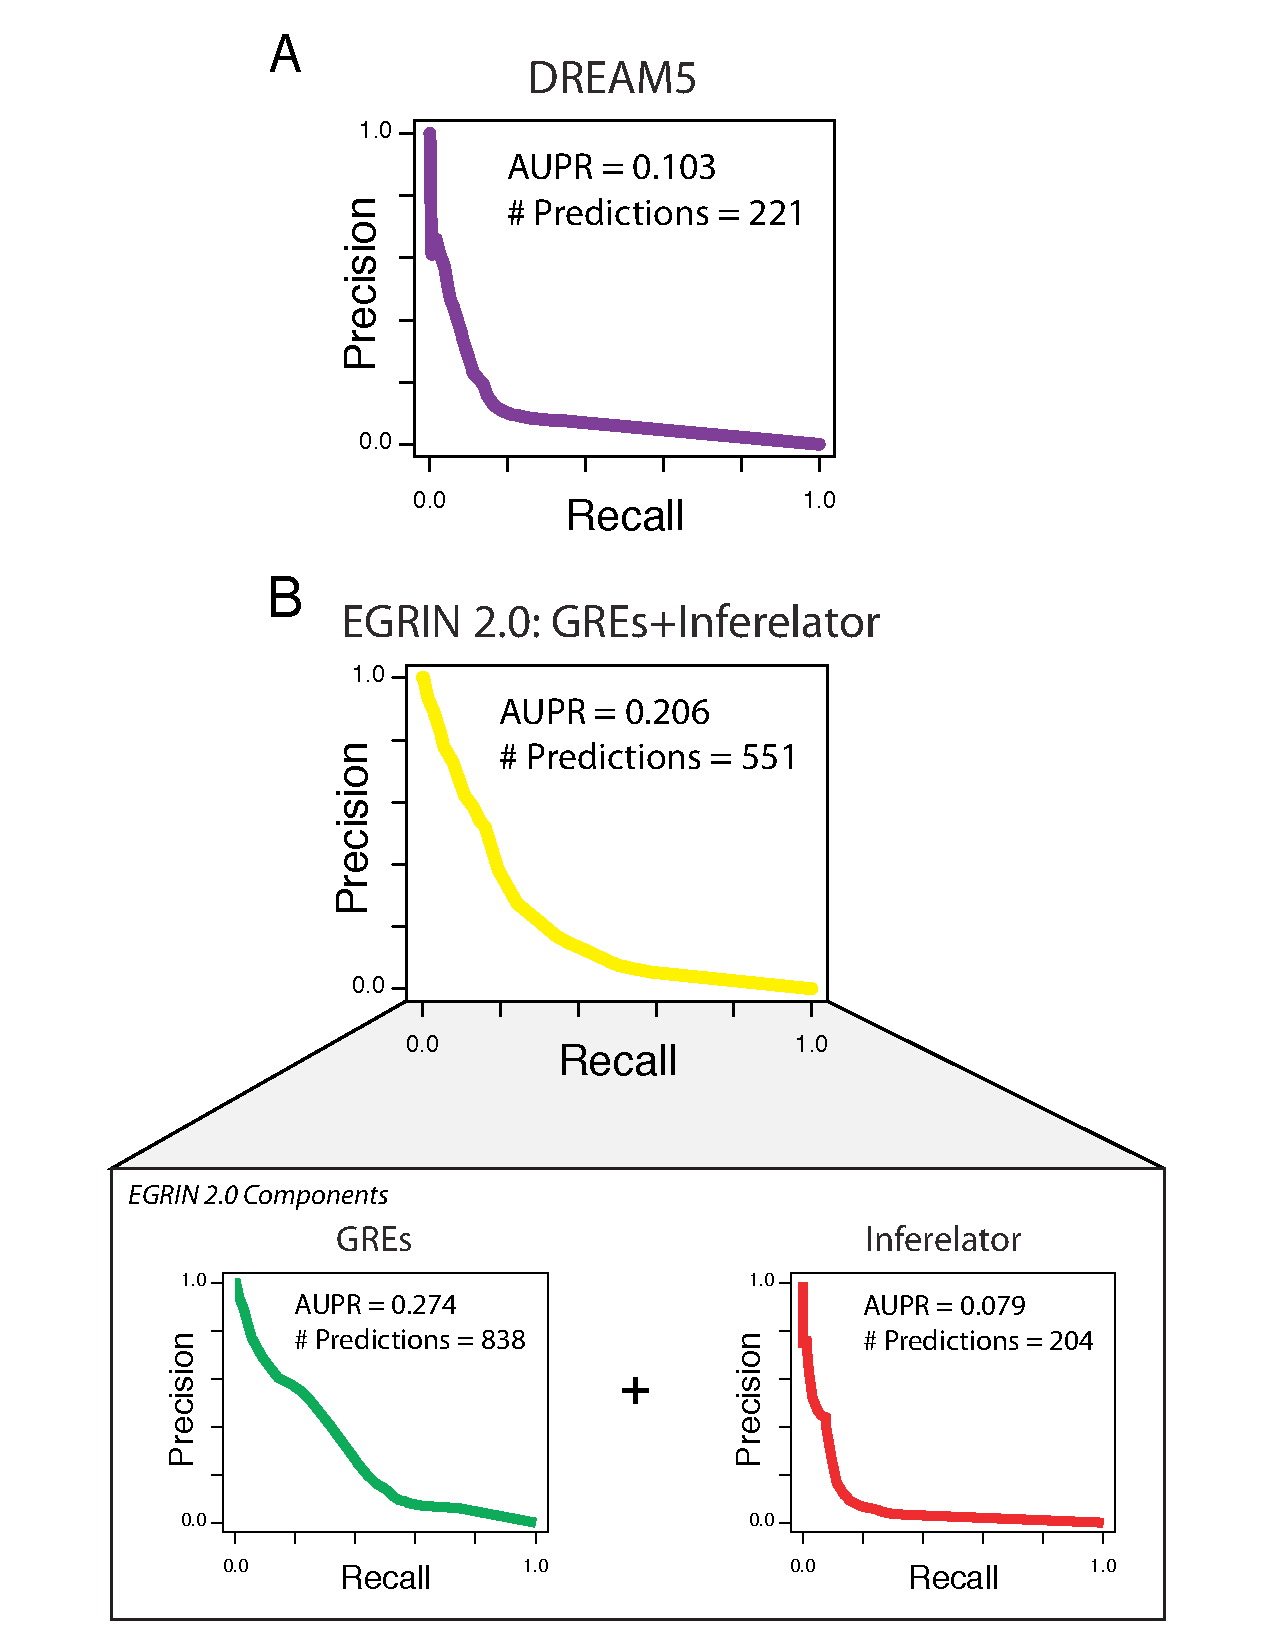
\includegraphics[width=0.5\linewidth]{figures/aupr.pdf}
\caption[Precision-recall performance for {\it E. coli}
  networks.]{\textbf{Precision-recall performance for \textit{E. coli}
    networks.} Comparison of precision-recall performance on {\it
    E. coli} \rdb~gold-standard (Section
  \ref{section:eco:gold:standard}), for the DREAM5 ensemble network
  (A), compared to \egrine (B).  We compare the GRE-based and
  \nwinf-based networks (bottom)to the integrated \egrine~network
  (top). The integrated \egrine~network consists of an equal weighting
  of the GRE-based and \nwinf-based networks.  The \egrine~networks
  were inferred using the DREAM5 mRNA expression compendium (Section
  \ref{section:dream5_data_compendium}). Area under the curve (AUPR)
  and the number of true-positive predictions at a precision of 25\%
  are listed for each curve.}
\label{fig:pr_curves}
\end{figure}

We further investigated the convergence of the AUPR statistics for
each of the \egrine-predicted regulatory networks as additional
individual EGRIN models are added to the ensemble. This assessment
helps to address the question of whether the approach utilized for
ensemble integration has the desired property of performing better
than most (if not all) of the individual models. Additionally, it can
address the question of how many individual EGRIN models are necessary
to achieve a given performance level. We observed that this is indeed
the case for the \nwinf-based predictions extracted from the
\egrine\ model (Figure~\ref{fig:cumulative_auprs}a), whose final AUPR
of 8.5\% far exceeds the rather poor performance of all 106 individual
component EGRIN models (with an average AUPR of 5.0\% and a maximum of
7.4\%). The performance of the ensemble for this measure converges
rather quickly to the final measure, after roughly 50 of the 106 EGRIN
models are integrated (taking into account the variance in models
observed with integrating the models in different orders).  For the
\egrine\ GRE-based predicted network
(Figure~\ref{fig:cumulative_auprs}b), ensemble surpasses 84 (79\%) of
the 106 individual component EGRIN models. This measure continues to
improve until $\sim 80$ of the 106 models are integrated, suggesting
that for this data set (the DREAM5 {\it E. coli} expression
compendium), $\sim 100$ EGRIN models was a reasonable number to use in
construction of the \egrine\ ensemble.

\begin{figure}[hp]
\centering
\mbox{
\subfigure[]{\includegraphics[width=0.4\linewidth]{figures/nwInf_cumulative_forPaper.pdf}}
\subfigure[]{\includegraphics[width=0.4\linewidth]{figures/motif_cumulative_forPaper.pdf}}
}
\caption[Ensemble performance of individual GRN predictions]{
  \textbf{Ensemble performance of individual GRN predictions.}
  \egrine-inferred \textit{E. coli} regulatory network predictive
  performance (AUPR vs. {\it E. coli} DREAM5 \cite{Marbach2012} gold
  standard) for \nwinf-based predictions (a) and GRE-based predictions
  (b) from \egrine. Shown for both networks is the cumulative AUPR as
  each of the 106 individual model components is integrated in to the
  ensemble (as described in
  Section~\ref{section:aupr:vs:regdb}). Lines showing the cumulative
  AUPR for randomized orderings of the components' integration into
  the ensemble reveal the slight variations in performance that could
  be observed, and that these converge prior to integration of the
  final ($106^{\text{\tiny th}}$) component. Also included for
  comparison is a box-whisker plot which shows the distribution of
  corresponding AUPR scores for the 106 individual EGRIN models. }
\label{fig:cumulative_auprs}
\end{figure} 

Figure \ref{fig:argR_purR_networks} shows the inferred networks for
two genes regulated by PurR and ArgR (comparing predictions from
\egrine, \tmsamp{CLR}, DREAM5, and \tmsamp{RegPrecise} to the
annotations in \rdb). The result demonstrates that GRE-based
approaches can discover interactions that are not predicted using
direct approaches (See Section~\ref{section:gre_grn_construction}).

\begin{figure}[hp]
\centering
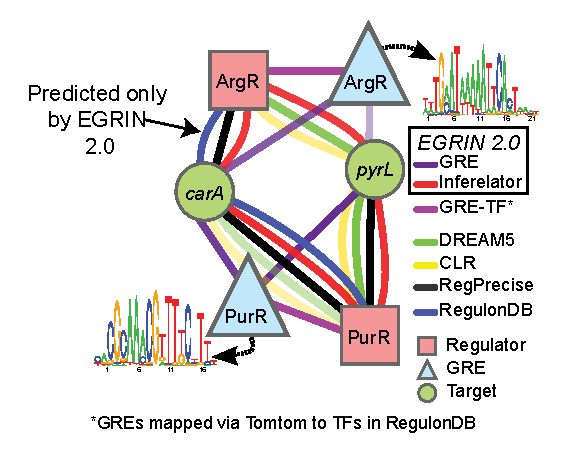
\includegraphics[width=0.5\linewidth]{figures/argR_purR_networks.pdf}
\caption[Integration of GRE discovery and \nwinf\ predictions
  yields comprehensive and detailed gene regulatory
  networks]{\textbf{Integration of GRE discovery and \nwinf\ 
    predictions yields comprehensive and detailed gene regulatory
    networks.} \egrine-inferred \textit{E. coli} regulatory subnetwork
  for two genes (green circles) in the PurR/ArgR regulon:
  \textit{carA} (\textit{b0032}) and \textit{pyrL} (\textit{b4246}).
  The \egrine~predictions are divided into GRE-based (dark violet) and
  \nwinf-based (red), and compared to predictions (or
  annotations) from other algorithms/databases (yellow: \tmsamp{CLR}; green:
  DREAM5 ensemble; black: \tmsamp{RegPrecise}; blue: \tmsamp{RegulonDB}). In two cases
  (ArgR$\rightarrow$carA and ArgR$\rightarrow$pyrL), \egrine~discovers
  regulatory interactions that were missed by either hand-curated
  databases or expression-based inference procedures.}
\label{fig:argR_purR_networks}
\end{figure} 

\subsection{Validation of condition-specific operon isoforms by tiling array transcriptome measurements}

We validated the prevalence of multiple, condition-specific
transcriptional isoforms from operons in \eco\ by measuring changes in
the transcriptome across growth, from lag-phase (OD600 = 0.05) to late
stationary phase (OD600 = 7.3). The experimental platform and other
experimental details are described in Section
\ref{section:ecoarray}. We used multivariate recursive partitioning,
including signals from both relative changes in expression along the
growth curve, as well as raw RNA hybridization signal to call putative
transcription breaks as previously described \cite{Koide2009}. To
determine the significance of our finding, we computed a $p$-value
describing the significance of the overlap between our predictions
(see Section \ref{section:condop}) and the experimental observations
using the cumulative hypergeometric distribution.

Figures \ref{fig:dpp_ecoli_expression}, \ref{fig:galE}, and
\ref{fig:ptsh} below depict several operons annotated with
condition-specific transcriptional isoforms. We have integrated GRE
elements discovered near break sites with the transcriptional
measurements.

\begin{figure}[hp]
\centering
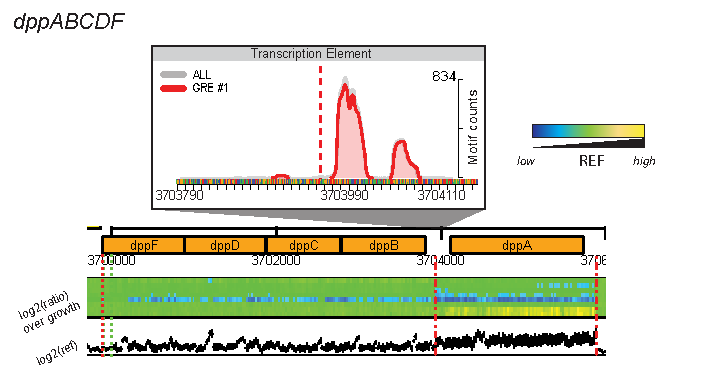
\includegraphics[width=0.7\linewidth]{figures/dpp_ecoli_expression.pdf}
\caption[GREs regulate multiple transcript isoforms from operons in
  {\it E. coli}, \textit{dppABCDF}]{\textbf{GREs regulate multiple
    transcript isoforms from operons in {\it E. coli},
    \textit{dppABCDF}.} GREs coincide with experimentally measured
  break sites. Three examples of experimentally determined
  transcription break sites (red dashed lines) in operons predicted by
  corems to be conditionally segmented. Expression levels of these
  regions were profiled across growth in rich media (heatmap). Inset
  contains region immediately surrounding a transcriptional break
  site, including counts of GREs discovered at these locations (as in
  Figure \ref{fig:nirH}).}
\label{fig:dpp_ecoli_expression}
\end{figure}

\begin{figure}[hp]
\centering
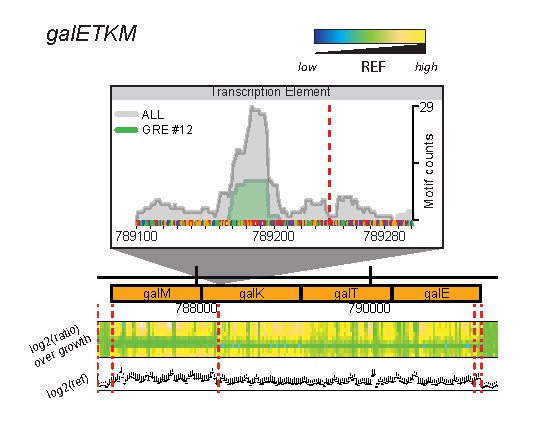
\includegraphics[width=0.7\linewidth]{figures/galE.pdf}
\caption[GREs regulate multiple transcript isoforms from operons in
  {\it E. coli}, \textit{galETKM}]{\textbf{GREs regulate multiple
    transcript isoforms from operons in {\it E. coli},
    \textit{galETKM}.} Caption details included in Figure
  \ref{fig:dpp_ecoli_expression}.}
\label{fig:galE}
\end{figure}

\begin{figure}[hp]
\centering
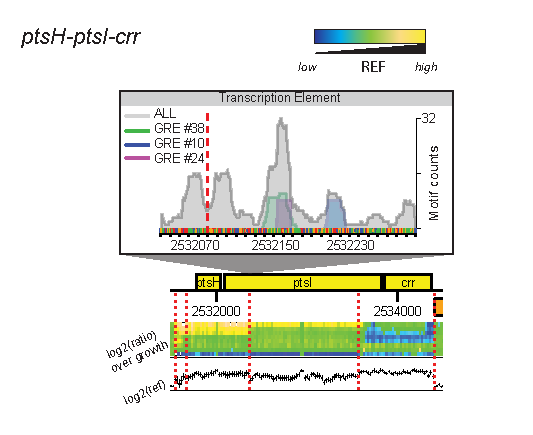
\includegraphics[width=0.7\linewidth]{figures/ptsh.pdf}
\caption[GREs regulate multiple transcript isoforms from operons in
  {\it E. coli}, \textit{ptsH-ptsI-crr}]{\textbf{GREs regulate
    multiple transcript isoforms from operons in {\it E. coli},
    \textit{ptsH-ptsI-crr}.} Caption details included in Figure
  \ref{fig:dpp_ecoli_expression}.}
\label{fig:ptsh}
\end{figure}

\subsection{Gene-gene co-fitness correlations in regulatory modules}

To assess the phenotypic consequences of co-regulation in corems, we
assessed whether genes grouped into corems had significantly similar
fitness consequences in many environments (\ie, the effect of deleting
one gene is highly similar to the effect of deleting the other across
many environments). We used the high-throughput fitness screen
described in Section \ref{section:fitness} to quantify these
relationships.

We compared the enrichment for high co-fitness relationships in corems
to other ways of assigning co-regulatory modules, including regulons
(\tmsamp{RegPrecise}, \rdb), operons, and \tmsamp{WGCNA}. The gene
modules for regulons (annotated in \rdb\ or \tmsamp{RegPrecise}
\cite{Novichkov2013}) consisted of genes annotated to a common TF. For
WGCNA, we assigned modules using the same community detection
procedures that we used to define corems from the \egrine~ensemble
(See \ref{section:gBg}). The gene co-expression modules were computed
from the weighted \tmsamp{WGCNA} adjacency matrix.

For the results presented in Figure~2B, we compared the distributions
of Pearson correlations between relative changes in fitness across
pairs of genes within each module, using the one-tailed
Kolmogorov-Smirnov test (KS-test). We report the KS $D$-statistic. The
precision/recall characteristics for each model are contained in Table~E5.

We extended this analysis by investigating whether the enriched high
co-fitness gene-gene relationships in corems consist of relationships
that could be described fully by regulons or operons. To answer this
question, we removed all gene pairs from corems that are also present
in operons or regulons and computed the KS-test again (Figure
\ref{fig:fitness_wo_operons}). We still observe a significant number
of high co-fitness relationships, suggesting that corems capture
physiologically meaningful co-regulatory relationships between genes
that cannot be explained by existing paradigms.

\begin{figure}[hp]
\centering
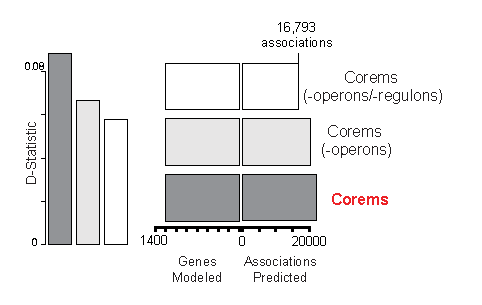
\includegraphics[width=0.6\linewidth]{figures/fitness_wo_operons.pdf}
\caption[\egrine~models highly correlated co-fitness relationships
  that cannot be explained by operons or
  regulons]{\textbf{\egrine~models highly correlated co-fitness
    relationships that cannot be explained by operons or regulons.}
  (Left) Enrichment for highly correlated, pairwise fitness
  measurements in gene knock outs across 324 conditions before and
  after removing gene associations annotated by operons
  (Microbes Online) and regulons (RegulonDB and RegPrecise)
  (KS-test,$D$-statistic). Two-thirds of gene-pairs with most highly
  correlated fitness within corems are not annotated by operons or
  regulons. (Right) Number of genes and associations predicted.}
\label{fig:fitness_wo_operons}
\end{figure}
